\documentclass[12pt, a4paper]{article}\usepackage[]{graphicx}\usepackage[]{color}
%% maxwidth is the original width if it is less than linewidth
%% otherwise use linewidth (to make sure the graphics do not exceed the margin)
\makeatletter
\def\maxwidth{ %
  \ifdim\Gin@nat@width>\linewidth
    \linewidth
  \else
    \Gin@nat@width
  \fi
}
\makeatother

\definecolor{fgcolor}{rgb}{0.345, 0.345, 0.345}
\newcommand{\hlnum}[1]{\textcolor[rgb]{0.686,0.059,0.569}{#1}}%
\newcommand{\hlstr}[1]{\textcolor[rgb]{0.192,0.494,0.8}{#1}}%
\newcommand{\hlcom}[1]{\textcolor[rgb]{0.678,0.584,0.686}{\textit{#1}}}%
\newcommand{\hlopt}[1]{\textcolor[rgb]{0,0,0}{#1}}%
\newcommand{\hlstd}[1]{\textcolor[rgb]{0.345,0.345,0.345}{#1}}%
\newcommand{\hlkwa}[1]{\textcolor[rgb]{0.161,0.373,0.58}{\textbf{#1}}}%
\newcommand{\hlkwb}[1]{\textcolor[rgb]{0.69,0.353,0.396}{#1}}%
\newcommand{\hlkwc}[1]{\textcolor[rgb]{0.333,0.667,0.333}{#1}}%
\newcommand{\hlkwd}[1]{\textcolor[rgb]{0.737,0.353,0.396}{\textbf{#1}}}%
\let\hlipl\hlkwb

\usepackage{framed}
\makeatletter
\newenvironment{kframe}{%
 \def\at@end@of@kframe{}%
 \ifinner\ifhmode%
  \def\at@end@of@kframe{\end{minipage}}%
  \begin{minipage}{\columnwidth}%
 \fi\fi%
 \def\FrameCommand##1{\hskip\@totalleftmargin \hskip-\fboxsep
 \colorbox{shadecolor}{##1}\hskip-\fboxsep
     % There is no \\@totalrightmargin, so:
     \hskip-\linewidth \hskip-\@totalleftmargin \hskip\columnwidth}%
 \MakeFramed {\advance\hsize-\width
   \@totalleftmargin\z@ \linewidth\hsize
   \@setminipage}}%
 {\par\unskip\endMakeFramed%
 \at@end@of@kframe}
\makeatother

\definecolor{shadecolor}{rgb}{.97, .97, .97}
\definecolor{messagecolor}{rgb}{0, 0, 0}
\definecolor{warningcolor}{rgb}{1, 0, 1}
\definecolor{errorcolor}{rgb}{1, 0, 0}
\newenvironment{knitrout}{}{} % an empty environment to be redefined in TeX

\usepackage{alltt}
\linespread{1}
\usepackage{graphicx}
\usepackage{lipsum}
\usepackage{verbatim}
\usepackage[vmargin=3cm, hmargin=2cm]{geometry}
\usepackage{url}
\usepackage{hyperref}
\usepackage{fancyhdr}
\usepackage{color}
\usepackage{amsmath, amssymb}
\usepackage{longtable}
\usepackage{lscape}
\usepackage{natbib}
\usepackage{xspace}
\usepackage{textcomp}
\usepackage{float}
\usepackage{booktabs}
\usepackage{subcaption}
% =======================================

% bibliography
\bibliographystyle{apalike}
\IfFileExists{upquote.sty}{\usepackage{upquote}}{}
\begin{document}
\tableofcontents
\newpage
\section{Introduction}
Cells are one of the fundamental units of life. They show an immense complexity and diversity. Their identity and function is determined by environmental stimuli, the physical environment, the cell cycle and neighbouring cells \citep{wagner2016revealing}. Only recently has it been possible to investigate the full transcriptome of a single cell. Single-cell RNA sequencing (scRNA-seq) was first published by \citet{tang2009mrna}. This method addresses new biological issues, such as the identification of rare cell populations, and allows us to measure the frequency of cell types in tissues, characterise differences in similar cell types and investigate the heterogeneity of cell states or cell lineages \citep{andrews2017identifying}.

A typical scRNA-seq workflow consists of the isolation of single cells, the extraction of RNA, cDNA library preparation, and the amplification and sequencing of the libraries. A wide variety of scRNA-seq protocols exists, differing in throughput, full transcript or 3' sequencing, costs and automatisation. Small-scale protocols are standard PCR plate-based methods or methods in which cell isolation and library preparation are combined into one protocol. A typical small-scale method is the PCR plate-based SMART-seq2 \citep{picelli2013smart}. Full-transcripts are sequenced using a standard Illumina approach. Typically, hundreds of cells are processed and spike-ins from the External RNA Control Consortium (ERCC) is used for normalisation. On the other side of the spectrum are droplet-based methods such as Drop-seq and 10xChromium, which allow the processing of thousands of cells.

The differences between scRNA-seq and bulk experiments are the lower sequencing depth (100,000--5 million reads per cell) compared to bulk experiments, higher variability and more outliers in the scRAnseq data. scRNA-seq data suffers from technical noise, batch effects and low capture efficiency. Confounding occurs when different biological conditions are processed in different batches, making the deconvolution of technical noise and biological effect impossible. This should be avoided by an appropriate experimental design that allows for the statistical deconvolution between unwanted and wanted variation. In scRNA-seq the single experimental unit is the cell, making it not always possible to use this approach. Different cells in an experiment may need different sample processing, or their biological differences may affect the downstream analyses.

The starting amounts of the library preparation can be as low as ten picogrammes of total RNA \citep{picelli2013smart}. Two main issues arising due to the low starting amount are  overamplification and low capture efficiency. Low and moderate expressed genes are not captured during the reverse transcription, which leads to dropouts of genes and a zero-inflated gene expression. scRNA-seq data has an excess of zero counts, which can be split into systematic, semi-systematic and stochastic zeros \citep{lun2016pooling}. Systematic zeros and semi-systematic zeros come from genes that are silent in a subpopulation or across all cells, respectively. 
Stochastic zeros are zero counts that have been obtained due to a low capture efficiency during the library preparation. They affect genes with a count distribution near zero and have to be dealt with the normalisation steps.  
 
To deal with technical noise Unique Molecular Identifiers (UMI) or spike-ins are used. UMI are short random barcodes attached to the single-stranded cDNA in the reverse transcriptase process. By counting the unique UMI reads aligned to the genome an estimated tag count is obtained. Spike-in are added before amplification. Under the assumption that the amplification of the endogenous and exogenous RNA is similar, they can be used for library size normalisation and to remove technical noise. 

In general, scRNA-seq experiments consist of high-dimensional data. High-dimensional data suffers from the curse of dimensionality \citep{wagner2016revealing}, which means the distances in high-dimensional data become unstable and subpopulations cannot be separated \citep{andrews2017identifying}. Additionally, computational requirements are high. Reduction of the dimension is made by two approaches. Using linear or non-linear projections of the data from the original high-dimensional to a lower-dimensional space, or by feature selection, in which uninformative genes are removed.

The characterizing of of the composition in a sample is one of the most common aims for scRNA-seq data. Lately, a broad spectrum of clustering methods have been specifically developed for the clustering of single cells. The aim of this study is to evaluate clustering methods for scRNA-seq data. 
\section{Methods}

\subsection{Dimension reduction}
All methods require a dimension reduction step before clustering. Commonly used methods are either Principal Component Analysis (PCA) or t-distributed Stochastic Neighbour Embedding (tSNE). PCA finds a rotation of the original data in which the newly obtained first coordinates have the highest possible variance, the second coordinates the second-greatest variance etc. Practically, PCA is computed by spectral decomposition of the correlation or covariance matrix. Dimension reduction is achieved either by selecting only the first few PCs whose eigenvalues are above the average, or by determining the number graphically by plotting the eigenvalues. PCA is deterministic and relatively fast but restricted to linear spaces.

In contrast,  tSNE is a non-linear mapping \citep{van2013barnes}. Stochastic neighbour embedding (SNE) transforms Euclidean distances to conditional probabilities $p_{j|i}$. That is the probability that \(x_j\) is the nearest neighbour of $x_i$ under a Gaussian centred at $x_i$. The low-dimensional counterpart $q_{i|j}$ is similar with a Gaussian centered at $y_i$ and variance of $1/\sqrt(2)$. SNE minimises the divergence between $p_{j|i}$ and $q_{j|i}$ using the Kullback-Leibler divergence. tSNE implements a Student's t-distribution for the low dimensional space and a symmetric version of the cost function to simplify optimisation and to overcome the crowding problem. In tSNE, the cost function uses the joint probabilities $p_{ij}$ and $q_{ij}$ instead of conditional probabilities. To deal with large datasets, the Barnes-Hut implementation uses random walks on the nearest neighbour network with a PCA step to reduce the dimensionality of the high-dimensional data. tSNE is stochastic, depends on a perplexity parameter and distances between clusters are not preserved. 
\subsection{Clustering methods}
Identifying unknown cell populations is one of the main uses of scRNA-seq data \citep{andrews2017identifying}. Eleven clustering methods have been evaluated for this study. These methods and algorithms can be roughly classified into three groups: K-means, graph-clustering and hierarchical-based clustering. 
SC3, SIMLR, Linnorm and RaceID use k-means in different fashions, while pcaReduce and CIDR are based on hierarchical clustering. The graph-based methods are SNN-Cliq and Seurat. An overview of the methods is given in Table \dots
\paragraph{K-means}
K-means clustering finds a predefined number of centres $k$ and cell assignments, such that their within-group sum of squares is minimised \citep{hartigan1979algorithm}. $k$ cluster centres are randomly assigned.
Each data point is then assigned to the nearest centre using Euclidean distances. The centres are then recomputed using the average of the data points that are assigned to each of the $k$ centres. This procedure is iterated until the algorithm converges. The assigning of the centres is random. Also, it's not guaranteed to find the global minimum.  The drawbacks of the method are that it assumes spherical clusters and this is sensitive to scaling. 
\paragraph{pcaReduce}
pcaReduce uses k-means clustering to find the number of clusters in the reduced dimension given by PCA \citep{yau2016pcareduce}. The main assumption is that large classes of cells are contained in low-dimension PC representation and more refined subsets of these cells types are contained in higher-dimensional PC representations. Given a gene expression matrix, the clustering algorithm starts with a k-means clustering on the PCA projections $Y_{n\times q}$ with $q+1$ clusters, where $n$ is the number of cells and $q$ are the number of PCs. The number of initial clusters $k$ is typically around 30,  guaranteeing that most cell types are captured. For all pairs of clusters, the joint probabilities are computed. Two clusters are merged by selecting the pair with the highest joint probability or by sampling proportionally by the joint probabilities. The number of clusters is now decreased to $k-1$. Next, the PC with the lowest variance is deleted and a k-means clustering with $k-2$ centers is performed. This process is repeated until only one single cluster remains. When using pcaReduce $q$ cluster partitions with $k-1$ clusters are obtained. The user can than choose the clustering with the desired number of clusters.
\paragraph{SC3}
Implemented in the SC3 method is gene- and cell-filtering, as well as a log transformation step of the expression matrix \citep{kiselev2017sc3}. The filtered expression matrix is then used to compute  Euclidean, Pearson and  Spearman dissimilarity measures. By PCA or Laplacian graphs a lower-dimensional representation of the data is obtained.  K-means clustering is then performed on the different dimensions. Next, a consensus matrix of the different clustering results is computed. The consensus matrix is a binary similarity matrix with entry one if two cells belong to the same cluster and zero otherwise. The consensus matrix is obtained by averaging the individual clustering. The last step is a hierarchical clustering step with complete linkage. The cluster is inferred by the $k$ level of hierarchy, where $k$ can be supplied by the user. The method allows for the estimation of $k$. (Using the covariance matrix of the expression matrix the function finds the eigenvalues. The Tracy-Widom test is used for estimating the number of significant eigenvalues, which represent the number of estimated $k$. )
To reduce runtime, SC3 changes the clustering method when supplied with more than 5'000 cells. Randomly selected cells are then used for the clustering approach described above. These subpopulations are then used to train a support vector machine to infer the cluster labels of the remaining cells.
\paragraph{SNNcliq}
SNNcliq computes a shared nearest-neighbour-graph based on the high-dimensional data \citep{xu2015identification}. The nodes are the data points and the weighted edges are the similarities between the data points. Cells are defined as a cluster if they have a defined number of edges between them, forming a "clique". 

A similarity matrix using Euclidean or other similarity measures is then computed. Using this similarity matrix, the k-nearest-neighbours (KNN) for each data point are listed. The number of nearest neighbours has to be supplied by the user. Edges between data points are assigned if they share at least one KNN. The weights of the edges are defined by a function of the number of nearest neighbours and their respective ranks. 
Identification of clusters is made by finding quasi-cliques associated with each node and merging them to unique clusters by the use of a greedy algorithm. A node induces a subgraph, which consists of all neighbour nodes and edges. For each node, a local degree is computed and a node is removed from the subgraph if its degree is lower than a given threshold which is proportional to the size of the clique. The threshold is supplied by the user and is typically set to 0.7. Next, the degrees between the nodes are recomputed and the process is repeated until no more nodes can be removed. A subgraph is assigned to a quasi-clique if it contains more than three nodes. To reduce redundancy, quasi-cliques that are completely included in other cliques are removed as well.
Clusters are then identified by merging the quasi-cliques. For each pair, an overlapping rate is computed. If it exceeds a predefined threshold $m$ the subgraphs are merged. Merging in different orders leads to different results, so pairs with larger sizes are prioritized.
\paragraph{SIMLR}
Most clustering methods rely on standard similarity metrics like Euclidean distances \citep{wang2017visualization}. SIMLR uses a weighted function of multiple kernels to compute a distance matrix. The assumptions is that the matrix has a block-diagonal structure, where the blocks represent the clusters $c$. The kernels are Gaussian kernels with a range of hyperparameters defining the variance of each kernel. The similarities are then used for data visualisation with tSNE or clustering using k-means on the latent space representations of the similarities.

\paragraph{CIDR}
Clustering through Imputation and Dimensionality Reduction (CIDR) takes the high dropout rate in scRNA-seq data into account \citep{lin2017cidr}. The method splits the squared Euclidean distance into three terms. These consist of one term in which both genes $k$ for the cell pairs $i$ an $j$ are non-zero, a second term in which one gene is zero and a third where both are zero. The authors state that only the cases where one gene is zero have a strong influence on the distances and the subsequent dimension reduction and clustering. To reduce the dropout-induced zero inflation, the method imputes the third term by its expected value given the distribution of the dropouts. 
The algorithm works basically in five steps: (i) Find features that are dropout candidates. That is genes that show an expression level below a threshold $T$. (ii) Find the empirical dropout probability $\hat P(u)$ using the whole data set. (iii) Calculate the dissimilarity using Euclidean distances together with a pairwise imputation process. Features that fall below the threshold $T$ are imputed using a weighting function. The weighting is based on the probability of being a dropout. (iv) Perform dimension reduction using PCA on the imputed distance matrix. (v) Perform hierarchical clustering using the first few PCs. The number of PCs can be determined by several methods. Here, we use an implemented variation of the scree method. 
\paragraph{Linnorm }
Linnorm is a normalisation and transformation method for count data \citep{yip2017linnorm}. The main assumption is that a homogeneously expressed gene-set exists. Using this gene subset, and by ignoring zero counts, the normalisation and transformation parameters are calculated. After normalisation, the expression values should show both homoscedasticity and normality. Linnorm includes functions for subpopulation analysis by t-SNE or PCA dimension reduction and subsequent k-means or hierarchical clustering. 

First, the values are scaled according to library size. Low count genes and genes that show high technical noise are filtered out. By default, genes showing a non-zero expression in at least 75 \% of the cells are retained. Note that this threshold is set to maintain at least three non-zero cells per gene, in order to calculate the skewness of the gene distributions. By gradually increasing this threshold only genes that show a negative correlation between the mean and the standard deviation (SD) is assured. 
A locally weighted scatterplot smoothing (LOWESS) curve is fitted on the mean versus SD relationship. The SD is scaled and outliers based on the SD are removed. Next, genes that show a high skewness are filtered out. The data is then transformed using a modified log transformation.
The dimensions are reduced by PCA or tSNE and clustering using the k--means algorithm. The R packages fpc, vegan, mclust and apcluster are used to determine the number of clusters.

\paragraph{TSCAN}
TSCAN uses a pseudo-time algorithm for cell ordering \citep{ji2015tscan}. PCA dimension reduction on the preprocessed gene expression data is performed. Preprocessing is done by log transformation and by adding a pseudo-count. Low expressed genes are filtered out based on the zero-proportion and their covariance. Clustering is done by model-based clustering. 
The travelling salesman problem (TSP) is then solved by a minimum spanning tree. The user can then define the start/end point through the available biological information and compute a pseudo-time ordering score. 
\paragraph{RaceID}
Rare Cell Type IDentification (RaceID) is a algorithm developped for the dat preprocessing, detection of outlier cells, kmeans clustering and the inference of rare subpopulations. Cells are filtered based on a minimum number of transcripts. The expression matrix is normalised by scaling by the library size. To ensure non-zero values a pseudocount of 0.1 is added to the expression data.
Using genefilter genes with a high zero-proportion are filterd out as well.
The implented clustering function uses k--means and the clusterboot function from the R package fpc for clustering. In contrast to the originial k--means clustering in clusterboot, the newly developped function can use not only euclidean distances. 
The number of clusters is determined by the use of the gap statistic implemented in the clusterboot function.

The authors state that the algorithm is based on absolute transcript counts and is not tested for datasets containing other expression values than counts. With respect datasets other than the Zheng data the results should be interpreted carefully.

\paragraph{Seurat}
Seurat uses raw counts, where filtering is both done gene- and cell-wise. A user-specified threshold for the minimum number of expressed features per cell and the minimum number of the  gene-wise expression per cell has to be defined. The counts from each cell are normalised by their total counts, scaled by a factor of 10000 and log-transformed. A set of high-variable genes (HVG) is found by calculationg the average expression and dispersion for each gene. Based on the average expression the genes are divided into bins. Within each bin z-scores for the dispersion is calculated. The HVG are then selected by their standart deviation.
Dimension reduction is done by PCA. The number of PCs is deterimed by a permutation test or graphically by plotting the eigenvalues of the PCs. Clustering is graph-based using a KNN-graph of the euclidean distances in the PCA space. Clustering of cells is done by SLM \ref{butler2017integrated}.

\newpage
\subsection{Datasets}
The datasets Kumar, Trapnell and Koh were downloaded from the \textit{conquer} repository \url{http://imlspenticton.uzh.ch:3838/conquer}. The Zheng data was downloaded from the 10xChromium repository: \url{https://support.10xgenomics.com/single-cell-gene-expression/datasets}. For the Kumar, Trapnell and Koh data count-scale Transcripts Per kilobase Million (TPM) are used.  These are on a count-scale and are independent from the average length of the transcript \citep{soneson2015differential}. The Zheng data consists of UMI counts.
\paragraph{\citet{kumar2014deconstructing}}
The Kumar dataset consists of $Dgcr8$-knockout and V6.5 variotypes from mouse embryonic stem cells (mESCs). Cells were cultured on a serum with a Leukaemia Inhibitory Factor (LIF) or under Erk and GSK3 signalling inhibition (2Li). The authors investigated the expression of pluripotency factors and their involvement in the heterogeneity of pluripotent stem cells. Sample preparation and whole transcriptome amplification was done using a Fluidigm C1 system and following a SMARTer protocol. Sequencing was done using the Illumina system with paired-end reads. Sequencing depth was 1 million reads per cell.
\paragraph{\citet{trapnell2014dynamics}} 
\citet{trapnell2014dynamics} used human skeletal muscle myoblast cells to investigate temporal differentiation. Cells were expanded under high--mitogen conditions. Differentiation was induced by switching to low-serum medium. Cells were captured before switching to low-serum medium (T0), after 24 h (T24) and 48h (T48). Between 49 and 77 cells were isolated at each time point and used for single mRNA-Seq library preparation by the use of a Fluidigm C1 system and following a SMARTer protocol. Libraries were sequenced with paired-end sequencing on a HiSeq 2500 (Illumina) platform. Sequencing depth was ˜4 million reads per library. The authors excluded libraries that contained fewer than 1 million reads. 
\paragraph{\citet{koh2016atlas} }
H7 human embryonic stem cells (hESCs) were used to study human mesoderm development. Starting from undifferentiated stem cells, several differentiation stages, sorted by time point and further refined by fluorescence-activated cell sorting (FACS) were isolated. Finally, nine different cell lines were obtained:  undifferentiated H7 hESCs (H7hESC), anterior primitive streak populations (APS), mid primitive streak populations (MPS), lateral mesoderm (D2LtM), FACS-purified DLL1+ paraxial mesoderm populations (DLL1pPXM), early somite progenitor populations (ESMT), PDGFRα+ sclerotome populations (Sclrtm) and two different dermomyotome populations (D5CntrlDRmmtm).
In total, ten different cell types were then sequenced on a Fluidigm C1 system and following a SMARTer protocol. Libraries were sequenced through paired-end sequencing on a HiSeq 2500 (Illumina) platform. Sequencing depth was 1 -- 2 million reads per cell. 
\paragraph{ \citet{zheng2017massively}}
FACS-purified fresh peripheral blood mononuclear cells (PBMCs) were used to assess the performance of the 10xChromium system. Sample preparation and library construction were done with a 10xChromium system. The libraries were sequenced using an Illumina system. For this study, the datasets for CD19+B, CD8+CD45RA+ naive cytotoxic, CD14+ monocytes and CD4+/CD25+ regulatory T cells were used to construct an artificial population. From each library, 200 cells were sampled before being merged to obtain a single expression matrix.
\paragraph{Simulated datasets }
Using the Splatter package, expression data were simulated \citep{oshlack2017splatter}. Parameters for the simulation were estimated from a subpopulation of the Kumar dataset.  Embryonic stem cell variotypes V6.5 with signalling inhibition and LIF were used for the estimation. SimDataKumar consists of 500 cells with four subpopulations. The fractions per subpopulations were 0.1, 0.15, 0.5 and 0.25 of the total cell population. The probability that a gene is differentially expressed is 0.05, 0.1, 0.2 and 0.4 in the four different groups. Similarly, SimDataKumar2 consists of four subgroups with fractions of 0.2, 0.15, 0.4 and 0.25 of a total of 500 cells. The fractions of differentially-expressed genes were lower, with a probability of 0.01, 0.05, 0.05 and 0.08. The spike-in RNA is excluded before the parameter estimation.


\begin{figure}
\centering
\begin{subfigure}{.5\textwidth}
  \centering
  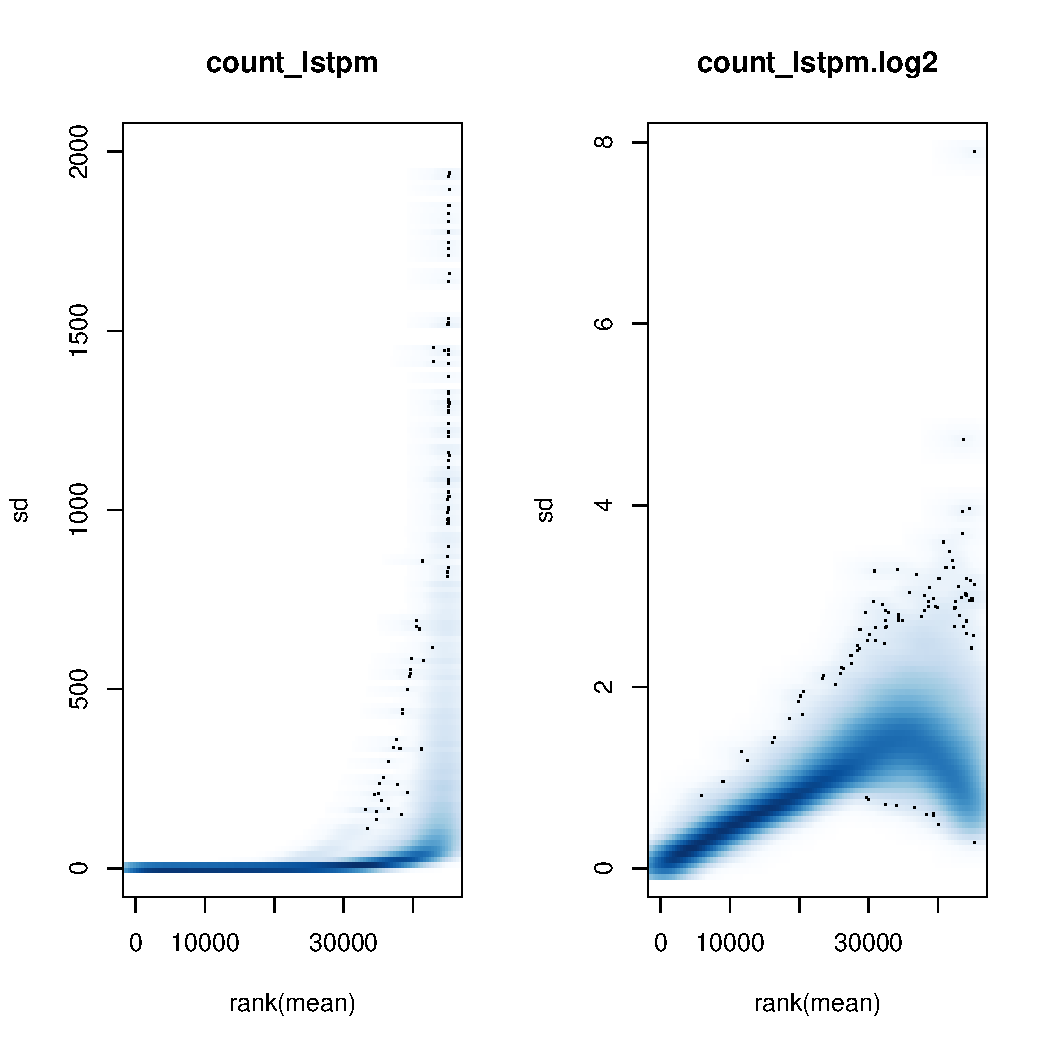
\includegraphics[width=1\linewidth]{/Users/angeloduo/Desktop/masterarbeit/scRNAseq_clustering_comparison/results/QC_data/meanvarplots_kumar2015.pdf}
  \caption{Kumar dataset}
  \label{fig:transsim}
\end{subfigure}%
\begin{subfigure}{.5\textwidth}
  \centering
  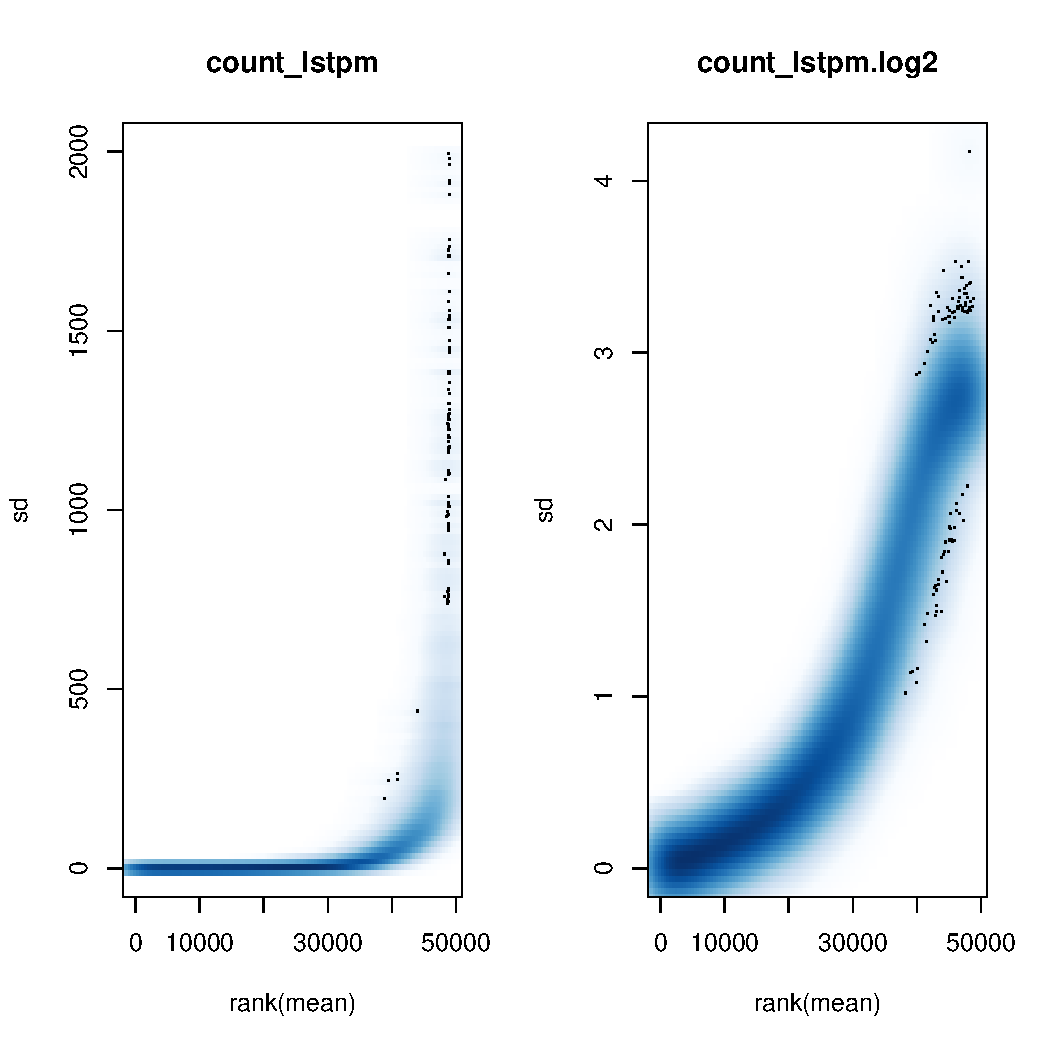
\includegraphics[width=1\linewidth]{/Users/angeloduo/Desktop/masterarbeit/scRNAseq_clustering_comparison/results/QC_data/meanvarplots_koh2016.pdf}
  \caption{Koh dataset}
  \label{fig:transkoh}
\end{subfigure}
\begin{subfigure}{.5\textwidth}
  \centering
  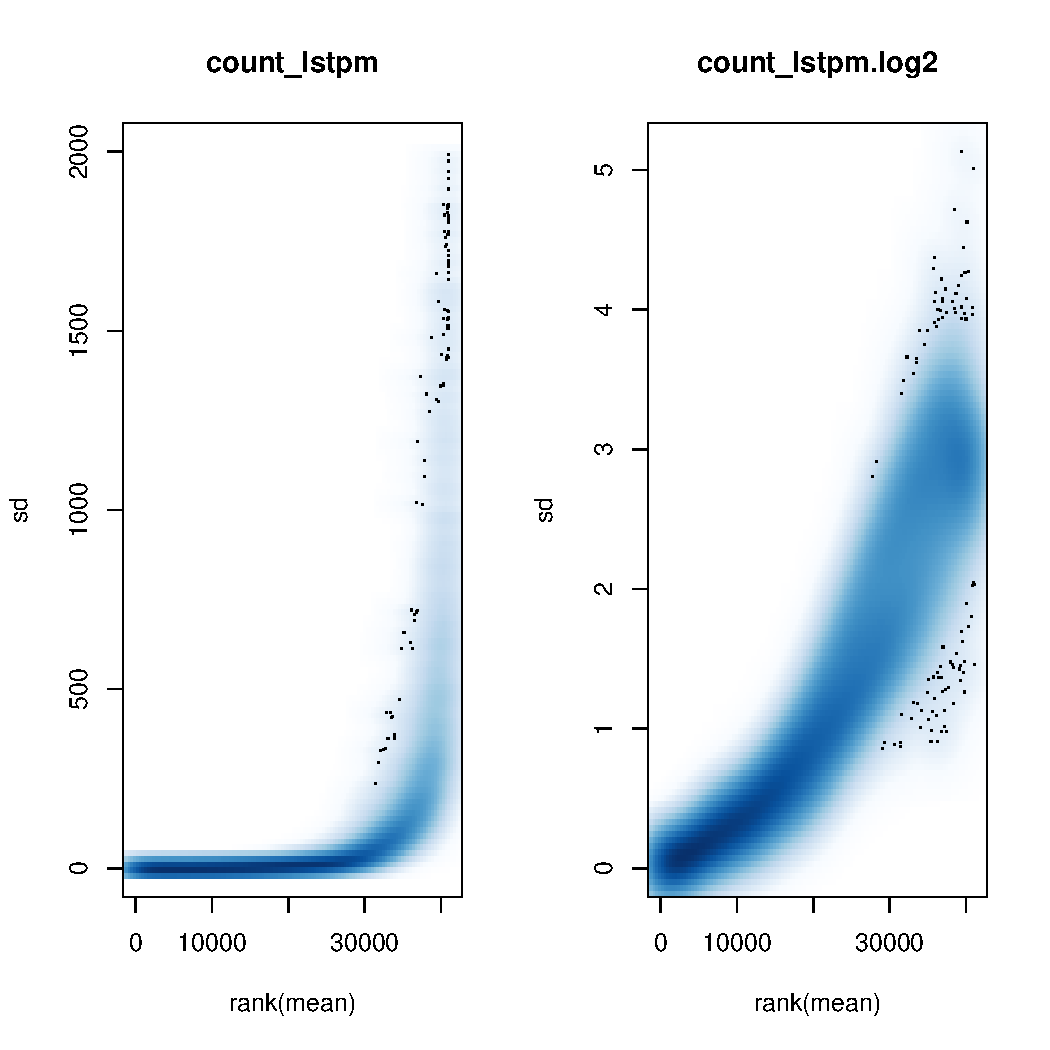
\includegraphics[width=1\linewidth]{/Users/angeloduo/Desktop/masterarbeit/scRNAseq_clustering_comparison/results/QC_data/meanvarplots_trapnell2014.pdf}
  \caption{Trapnell dataset}
  \label{fig:transtrapnell}
\end{subfigure}%
\begin{subfigure}{.5\textwidth}
  \centering
  \includegraphics[width=1\linewidth]{/Users/angeloduo/Desktop/masterarbeit/scRNAseq_clustering_comparison/results/QC_data/meanvarplots_zhengmix2016.pdf}
  \caption{Zheng dataset}
  \label{fig:transzheng}
\end{subfigure}
\caption{Shown is the genewise standart deviation versus the mean for the datasets Kumar (a), Koh (b), Trapnell (c) and Zheng (d). Different transformations were considered; log, arcus sin and VST transformations. }
\label{fig:trans}
\end{figure}

\newpage
\subsection{Data transformation and normalisation}\label{ssec:norm}
\paragraph{Data transformation}
RNA-seq data may suffer from heteroscedasticity and skewness \citep{zwiener2014transforming}. Genes with higher mean have on average a higher variance across cells leading to unequal variances between different genes. 
To handle this property different transformation were considered. Namely, a binary logarithmic transformation with a pseudo-count of one, arcus sinus transformations and a variance-stabilising transformation (VST) from the DESeq package \citep{huber2002variance}. Log transformations will have an impact on extreme values. However, they will not address the problem of heteroscedasticity. Arcus sinus transformation should deal with extreme values and equalise the variances. After transformation, the mean and the variances should be independent. VST addresses the problem of extreme values and unequal variances across genes. After such transformation, the mean and the variances of the genes should be independent. For the study, a binary logarithmic transformation plus a pseudo-count of one is used.  The mean-SD dependence for different transformations is shown in Figure \ref{fig:trans}.

\newpage
\paragraph{Filtering and normalisation}
The quality control of the data sets follows \citet{lun2016step}. In the first step, genes that are not expressed in any cell (systematic--zeros) are removed in order to reduce the size of the expression matrix. To find potential outliers, PCA can be used on the phenotype characteristic of each cell (Figure \ref{fig:qckumar}, \ref{fig:qctrapnell}, \ref{fig:qckoh}, \ref{fig:qczheng}; a). Cells were filtered based on the library size and the total number of genes.
Cells with log10 library sizes that are more than three median absolute deviations (MADs) below the median log-library size were filtered out (Figure \ref{fig:histkumar}, \ref{fig:histtrap}, \ref{fig:histkoh} and \ref{fig:histsim}). The same filter was used with respect to the total number of genes per cell. 
For the Kumar and the Zheng dataset, ERCCs and mitochondrial counts were available. Cells with large proportions of ERCC or mitochondrial RNA are seen as low-quality cells. In the Kumar dataset, cells with an median ERCC proportion above three MADs are as well removed. The same filter was used for mitochondrial RNA in the Zheng data.

The metadata for the Trapnell dataset contained information about the cell quality. In this dataset, cells that were marked as debris and any single libraries consisting of more than one cell were filtered out. After filtering, 531 cells in the Koh dataset, 246 in the Kumar dataset and 222 in the Trapnell dataset were retained. The filtering was less strict in the Koh dataset compared to the original analysis where they retained 498 cells. 

Low-abundance genes influence the mean-variance trend. Here low-abundance genes are filtered by their average counts (see Figures \ref{fig:qckumar}, \ref{fig:qctrapnell}, \ref{fig:qckoh} and \ref{fig:qczheng}; d ). For the Kumar, Trapnell, simDataKumar and Zheng data genes with average counts less than one are removed. The Zheng data set had a shallower sequencing depth. A different filter is used, and features which are not expressed in at least two cells are excluded.
To find batch effects, a linear model regressing the PC values against the total features was used \citep{lun2016step}. 

Another examination of the technical variation was done using the marginal variances\citep{lun2016step}. For that, a linear model with the expression values per gene as response variables and a chosen explanatory variable is fitted. The correlation coefficient can then be seen as the marginal explained variance for the explanatory variables.

A wide variety of normalisation methods exist based on bulk RNA methods. These methods are usually not designed for dealing with the zero-inflated nature of scRNA-seq data \citep{lun2016pooling}. 
Methods for normalisation of scRNA-seq data are based on spike-ins or RNA counts. Spike-in RNA is added before the library preparation. Any changes in the spike-in coverage are assumed to be due to technical factors. The normalisation is done by scaling the counts to level the spike-in. However, this approach is not feasible as none or only a limited number of spike-in counts were present in the datasets.

Here, normalisation through pooled cells is used, where the problem of excess zero counts is reduced by the pooling of multiple cells \citep{lun2016pooling}. The normalisation procedure can briefly be described as follows: (i) Different pools of cells are defined. (ii) The expression values are summed across the cell pools. (iii) The cell pool is normalised against an average of the summed expression values. (iv) This step is repeated several times to construct a linear system. 
The summed count size is then used to estimate the corrected size factor. The size factors for the pooled cells are then deconvoluted" into cell-based factors. 





\subsection{Optimal number of clusters}
Methods to determine the optimal number of clusters are subjective methods as elbow or silhouette plots. In the Elbow plots, the within-cluster sum of square is plotted against a range of clusters. The silhouette plot is a standardized measure of distances between each point inside and outside of the respective cluster. Less subjective is the gap statistic. Here the log within sum of squares is compared to its expectation. The null distribution is expected to be uniformly distributed, it is not clear if this is correct for high dimensional data \citep{tibshirani2001estimating}. Other possible methods are the calinsky criterion, hierarchical clustering....
Here the optimal number of clusters is determined by Elbow plots, clustering is based on kmeans clustering and the within-cluster sum of square thereof.
The elbow plots suggest three clusters for the Kumar dataset, 2 - 5 in the Trapnell data, 3 in in the Zhengmix data (see Figure \ref{fig:transkumar} ). The optimal number of clusters is unclear for the Koh data set. 
Minimization of within sum of squares was also done in the tSNE latent space with 30 dimensions. Here the optimal number of clusters are 3,3, 4 and 6 to 8  in the Kumar, Trapnell, Zheng and the Koh data sets, respectively.

\newpage
\subsection{Evaluation of the clustering methods using different run modes}
Using filtered and normalised data, the methods were operated in the default mode, with the number of clusters given by the ground truth and under a range of parameters. Additionally, the methods were also run with the unfiltered datasets. 

Many users will use these methods in the default mode, hence it was seen as important that the results were provided without any fine-tuning of the parameters.
The run parameters in the default mode were given either according to the packages default settings or by using examples from the package vignettes. If the method was able to detect the number of subpopulations, this auto-detection function was used to infer the number of clusters. When the number of clusters had to be provided, the number of clusters given by  authors of the datasets were used. Clustering results have to be evaluated using some sort of "ground truth". Here, the cell annotation provided by the authorsof the datasets or the the given truth from the simulations were used.

Seurat, TSCAN, RaceID, SC3 and Linnorm each have their own filtering and/or normalisation procedures. In order to test these methods preprocessing capabilities, the methods were tested with the unprocessed raw counts.
The methods tSNEkmeans, pcaReduce, SNN-Cliq, SIMLR, ZinbWaVE and CIDR do not include filtering and normalisation steps. For these methods filtered, normalised and log-transformed counts, detailed in section \ref{ssec:norm}, were used. An overview of the filtering and normalisation steps used by the methods is given in Table \ref{tblone}.

In a further analysis, the clustering methods were tested for different values of the number of clusters $k$. Seurat does not allow the number of clusters to be set. Hence, Seurat was run under a range of the parameters of the number of neighbors and the resolution parameter.

Based on the evaluation by the Adjusted Rand Index (ARI), the parameter $k$, which maximises the ARI score was used to compare the methods in an optimal setting. To assess the stability of the clustering methods, a random subsample of cells without replacement was drawn from the Kumar dataset. The size of the subsample was 100 and the subsampling was repeated 30 times. The clusterings for each method were then compared using the overlapping samples and the ARI scores.  


\subsection{Parameter settings}
The number of clusters $k$ is the main parameter used for most of the methods. Except for Seurat, the clustering functions for each of the methods allow for the number of subpopulations to be directly controlled. Seurat allows the setting of $k$ only indirectly through a resolution parameter. 
The other important parameters were the number of kNN, the number or the type of latent space dimensions used for the clustering algorithms and the settings of the filtering and normalisation steps. The methods pcaReduce, SC3, Linnorm, RaceID and TSCAN can be run in an unsupervised mode, and no parameters have to be provided. Although it is possible to run these the methods unsupervised, fine-tuning of the parameters is highly recommended. CIDR, RtSNEkmeans and SIMLR need the specification of the number of clusters $k$.
For Seurat the number of PCs or the number of the kNN have to be defined. 
Next, a brief overview of the chosen parameter setting and the rationale behind it is given.
\paragraph{RtSNEkmeans}
To reduce the run time the Barnes-Hut tSNE implementation from the R package Rtsne was used. Perplexity was set to 30 for all datasets. Different values of the perplexity can give different tSNE representations; however, here the default setting with the perplexity parameter set to 30 was chosen. tSNE is performed on the first 20 dimensions in the PCA latent space. 
\paragraph{pcaReduce}
For pcaReduce, the range of clusters cannot be specified. Instead, the number of dimension $q$ in the PCA latent space are to be specified. The results are $q-1$ different clustering solutions, with $k-2$ clusters. For all data sets, 30 dimensions were chosen, and the evaluation was based on the respective number of clusters in the subsequent analysis. The method is stochastic and has to be run several times in order to give stable results. Here, 100 samples were chosen and the merging of clusters was done by sampling that was proportional to the joint probabilities. 
\paragraph{SC3}
A gene-filtering step is implemented in this method. Based on the dropout distribution, genes that are below the 10th and above the 90th percentile are filtered out. However, for the Koh and Zheng datasets the upper threshold is set to the 99th percentile. Due to the high dropout rate in these datasets, it was otherwise not possible to run the method .
When running under the default mode, a range of clusters from 2 to 10 are given, and the number of subpopulations is automatically inferred by the method. Otherwise, $k$ is set to the number of annotated subpopulations. 
\paragraph{SIMLR}
A gene-wise mean normalisation step is implemented by the method. When running in the default mode, no normalisation was used. However, in the other run modes normalisation was included. Without normalisation, the method fails in the spectral decomposition of the similarity matrix. 
The tuning parameter $k$ was set to the default value of 10 on all runs. The number of clusters is set according to the run mode that is being used.
\paragraph{CIDR}
CIDR uses three parameter settings: the number of clusters, the number of PCs (nPCs) and the method for hierarchical clustering. By default, Ward linkage are used in the hierarchical clustering. CIDR is able to automatically detect the the number of clusters $n$. By default, $n$ is set to $nPC*2+2$ and the parameter nPC is set to 4 by default. When run in a mode other than the default, the parameter nPC was chosen by a variation of the scree-plot and the number of clusters was set accordingly to the respective dataset. 
The number of PCs used for the datasets Kumar, Trapnell, Koh, Zheng, simDataKumar and simDataKumar2 are  5, 10, 8, 8, 3, and 3, respectively.

\paragraph{Seurat}
Implemented in the method is a normalisation and a gene-filtering step. The filtering criteria are based on how many cells show an expression of a certain gene and the number of total features per cell. By default, no cell-filtering step is included when preprocessed datasets are used.

When running with unfiltered data, genes that are expressed in less than two cells were filtered out. When using the Zheng data, the threshold is set to one, according to the filtering detailed in section \ref{ssec:norm}.

The default log normalisation is used, which is currently the only option. The scale factor for cell-level normalisation was set to the default of 10'000. 
As a default, no explanatory variables were chosen to be regressed out. The experimental batch would be a natural choice as a covariate, but it cannot be used as the datasets containing this information are completely confounded.

The clustering parameters to be defined were a resolution parameter and the number of PCs. The resolution parameter was set to 0.7 for the Koh dataset and 0.6 for the other datasets. 
The number of PCs was determined according to the methods recommended by the authors. Namely, through the use of a scree plot and a jackknife permutation test the number of PCs was determined. 
In terms of the datasets, Kumar, Trapnell, Zheng, Koh, simDataKumar and simDataKumar2 were used, with the number of PCs being  9, 12, 10, 15, 10, and 10, respectively.
Ten percent of the total cells were used as the number of neighbours in the k-nearest neighbour algorithm.  A range from 0.5 \% to 40 \% of the total number of cells is used to infer the optimal number for the kNN parameter.


\paragraph{TSCAN}
TSCAN adds a pseudo-count of one with the data being log-transformed; this setting is used for all run modes. 
In the default run-mode, genes that show zero expression in at least half of the cells are filtered out. In order to be able to run the method using the unfiltered data, this threshold was changed to 0.1 for the Zheng, simDataKumar and simDataKumar2 data.

This filter was switched off when working with the prefiltered datasets. By default, the method infers the number of clusters from a range of 2 to 9 clusters. Here, a range from 2 to 10 was used in the default mode. If run semi-supervised, the respective number of clusters is given. By default, "ellipsoidal, varying volume, shape, and orientation" is used for the model.

\paragraph{SNNCliq}
The connectivity of the quasi-cliques was set to the default value 0.7. Likewise, the merging threshold parameter was set to the default of 0.5. The method was run using normalised, filtered data and the number of clusters was set to a range from 3 to 10 in all datasets. SNNCliq works on different distance metrics; here, the default Euclidean distances were used.

\paragraph{RaceID}

In default mode, cells with a minimum total library size of 3'000 are retained. The gene filter is set to filter out all genes with less than five transcripts in at least one cell. Oversaturated genes, that have over 500 transcripts per cell, are also filtered out. Here, we only use this filter with the Zheng data, as it is the only set that contains UMI counts. Otherwise, the filter is turned off. The gap statistic is used to determine the number of clusters. The default setting from the clusterboot function is set to a range from 2 to 20 clusters.

When using the run mode with unfiltered datasets, the minimum total library size was set to 1'000, 500, 400, 420, 1'200 and 1200 for the datasets Kumar, Trapnell, Koh, Zheng, simDataKumar, and simDataKumar2, respectively. These thresholds were chosen so that they corresponded with the thresholds based on the MADs. The filters for oversaturated genes and minimum gene expression were turned off as well, corresponding to the filtering steps in section \ref{ssec:norm}.
Filtering, based on the original analysis, was done using mean counts. To set the gene filter, we retained those genes that showed at least one transcript for two cells in the count-based datasets. The exception to this was the Zheng dataset, where genes are retained that show at least five counts in two cells. 

When the method is run with prefiltered datasets, the filters are turned off and the appropriate number of clusters is provided. 
In all run modes, the Pearson metric is used as the distance measure.  

\paragraph{Linnorm}
Except for the  Zheng data, the filtering thresholds are set to the default in all run methods. Due to the low sequencing depth of the Zheng dataset, the minimum non-zero expression had to be set to a proportion of 0.1. tSNE and k-means are used for dimension reduction and clustering, respectively. In the default run mode, a range of $k$ from 2 to 20 was provided in order to allow us infer $k$.
\subsection{Evaluation metrics}
One of the evaluation criteria used was the Hubert-Arabje Adjusted Rand Index (ARI), which is used to compare two partitions \citep{hubert1985comparing}. The metric is adjusted for chance by subtracting the uncorrected index by its expectation, and divided by a scale factor. Independent clusterings have an expected value of zero and are one if there is full agreement between the partitions. The index can take on negative values.

Another metric is the F1 score. It is the weighted average mean between precision and recall. The weights are defined as the inverse of the precision and recall. F1 scores can take on values between zero and  one. The predicted clusters and the "ground truth" were matched by the Hungarian algorithm. Some of the clustering methods are unsupervised and the partitions do not need to have the same sizes ( non-bipartite ). This causes problems with the Hungarian algorithm. As a solution to this issue, the assignment matrix was augmented with dummy columns that had the maximum matrix value as their entries.



% latex table generated in R 3.4.2 by xtable 1.8-2 package
% Tue Jan 16 15:55:15 2018
\begin{table}[ht]
\centering
\begin{tabular}{rlllll}
  \hline
 & cellfiltering & genefiltering & normalization & autodetect & expressionvalues \\ 
  \hline
tSNEkmeans & no & no & no & no & normcounts \\ 
  pcaReduce & no & no & no & no & normcounts \\ 
  SC3 & no & yes & no & yes & normcounts \\ 
  SNNCliq & no & no & no & no & normcounts \\ 
  dbscan & no & no & no & no & normcounts \\ 
  SIMLR & no & no & yes & no & normcounts \\ 
  CIDR & no & no & no & yes & normcounts \\ 
  Seurat & yes & yes & yes & no & counts \\ 
  TSCAN & no & yes & yes & no & counts \\ 
  ZINBWaVEkmeans & no & no & yes & no & counts \\ 
  RACEID & yes & yes & yes & yes & counts \\ 
  Linnorm & no & yes & yes & no & counts \\ 
   \hline
\end{tabular}
\caption{Overview of filtering and normalization steps by method} 
\label{tblone}
\end{table}


\clearpage

\section{Results}

\subsection{Transformation and normalisation}

In Kumar similar amount of the variance is explained by the total number of genes, the proportion of ERCC and the phenotype. This indicates that the data set is heavily influenced by batch effects. The same holds in the Trapnell data, but on a lower scale. Variance in Koh data is primarily influenced by the phenotype and to a lesser extent by the total number of genes and the top 200 features. 
Zheng is primarily dominated by the biological variation with the other explanatory factors contribution only marginally to the total variances.
(Different methods exist to normalize RNA-seq data like TMM normalization, DEseq normalization and by library size. However, none of these methods is designed to deal with the zero-inflated nature of scRNA-seq data \citet{lun2016pooling}.
Another often used approach for scRAN-seq data is the normalization by spike-inn. This approach is not feasible as no or only a limited number of spike-inn counts were present in the data sets.)
The data still shows heteroscedasticity. There are only subtle differences between the arcus sinus and log transformations in all the datasets. The Compared with the Arcus sinus transformation.

\subsection{Evaluation of the clustering results}
\begin{figure}[!h]
\includegraphics[width=7 in]{/Users/angeloduo/Desktop/masterarbeit/scRNAseq_clustering_comparison/results/plots/plot_ari_all.pdf}
\caption{ARI scores for the datasets Koh, Kumar, Trapnell, Zheng and the simuations simDatakumar and simDataKumar2. Shown are the ARI scores for the runmodes (a) default, (b) filtered, (c) unfiltered and (d) optimalk. }
\label{fig:ariall}
\end{figure}

\begin{figure}[!h]
\includegraphics[width=5 in]{/Users/angeloduo/Desktop/masterarbeit/scRNAseq_clustering_comparison/results/plots/plot_ari_rank_all.pdf}
\caption{Ranks of ARI scores.  }
\label{fig:arirank}
\end{figure}



\begin{figure}[!h]
\includegraphics[width=5 in]{/Users/angeloduo/Desktop/masterarbeit/scRNAseq_clustering_comparison/results/plots/plot_ari_diff_maxscore_all.pdf}
\caption{Differences between maximum ARI scores.  }
\label{fig:aridiff1}
\end{figure}


\subsection{Evaluation of the clustering results}

The ARI scores for the different run modes are shown in Figure \ref{fig:aridef}, \ref{fig:ariunfilt}, \ref{fig:arifilt} and \ref{fig:ariopt}. The ranking of the scores for each method is shown in Figure \ref{fig:arirank}. The clustering methods showed highly varying accuracies, depending not only on the datasets, but also based on the run modes.  By running the clustering methods using the unfiltered and filtered datasets, we can (to some extent) investigate the effect of the filtering steps on the clustering. Figure \ref{fig:aridiff1} shows the differences between the method with the highest ARI score and the other methods, according to the dataset used. The methods SC3, SIMLR, ZINB-WaVE and CIDR all show higher ARI scores when the filtered datasets are used. No definite statement can be made about the performance of tSNEkmeans, as this method gives unstable results. RaceID, Linnorm, TSCAN and Seurat each have their cell or gene-wise filters implemented; these were included when running using the unfiltered datasets. Otherwise, they were deactivated. Linnorm, Seurat and RaceID showed similar or higher ARI scores when the pre-filtered datasets were used. Especially for the Koh dataset, the filters or the parameter settings seemed insufficient. 

By running the datasets in default mode and with a refined parameter, it is possible to investigate how to set the influence to allow for fine-tuning (see Figure\ref{fig:aridiff1} ). Note that the number of parameters varied considerably between the methods; in this study, we chose only the parameter that is regarded as the most important. For those methods with a filtering step, all the parameters set that defined the filtering process were changed. Linnorm, RaceID, SC3, Seurat, SIMLR, and ZINB-WaVE all showed an improvement or similar results when running with changed parameters. In the case of pcaReduce and tSNEkmeans, the results were not so clear, probably due to the stochasticity of these methods. In the default mode, the methods SIMLR, TSCAN and RaceID failed to cluster some of the datasets. 


The methods with generally high accuracies are SC3, Seurat and CIDR. These three methods showed higher ARI scores over all datasets and in the run modes, in comparison with other clustering methods. In general, pcaReduce and RaceID showed low ARI scores. As stated above, the accuracies varied between the run modes.
SC3 showed higher or similar ARI scores for most of the run modes, compared to Seurat and CIDR. The only exceptions are seen in the default setting when using simDataKumar2, Trapnell, and Zheng datasets. A pre-filtering step and a fine tuning of the parameters for this method is recommended, as this improved the accuracy of the method. 

The performances between Seurat and SC3 when used with the Kumar, simDataKumar and simDataKumar2 datasets were similar. However, Seurat’s performance levels dropped when used with the Koh and Zheng datasets. According to \citep{butler2017integrated}, the resolution parameter  for the function is crucial to the ability to determine the number of clusters, and it is recommended that the method be tested using different values of this parameter. In this study, we were only able to run the methods on a small range of values in the parameter, as else it was not possible to run the method. However, two of the tested values (0.6 and 0.7) mostly achieved good results. The filtering of the Koh dataset led to an improvement in the accuracies, but otherwise no or only small changes were detected.  
 
The default for the number of neighbours in the kNN method is set to 30, and no differences in the clustering is achieved when this parameter was set to 10 percent of the dataset. 

Although CIDR showed an overall high level of accuracy, it had one of the lowest performances for the Zheng dataset of all the methods tested. A possible reason for its low performance is that the expression values are UMI counts and the data has a low sequencing depth, leading to a wrong model fit in the imputation procedure. Filtering improved this method’s performance. We attempted to further improve this method’s performance by selecting an appropriate number of PCs; however, no improvements in accuracy were achieved. 

The method tSNEkmeans achieved similar accuracies compared to the high-performing methods when used with the simple Kumar, simDataKumar, and Zheng datasets, but it showed consistently low accuracies for the Koh dataset. When run under the optimal setting with the optimal number of clusters, the method achieved similar accuracies than SC3, but failed to correctly cluster the Koh dataset. 

The k-means algorithm assumes spherical clusters, which, in the tSNE representation of the dataset Koh, are not given. When comparing the different results achieved when using tSNEkmeans in the different run modes, the method gives unstable results. A possible reason for this is the stochastic nature of the k-means and tSNE algorithms. 

In comparison to the other methods, SIMLR achieved only high performances for the simple SimDataKumar and the Zheng dataset. Filtering the datasets led to an improvement for the Trapnell dataset, but otherwise had only a slight impact. A mean scaling of the data is recommended, or else the method was not able to cluster several of the datasets. 

Linnorm had relatively high accuracies for the unfiltered Trapnell and Zheng datasets. This could be due to the filtering functions that are implemented in the method. However, the method was highly unstable, and the results for the different run modes are not comparable. 

pcaReduce showed a unstable behaviour when running the method repeatedly. It achieved the highest accuracy for the Zheng dataset under the setting with the optimal number of clusters, but otherwise had low accuracies. The filtering of the datasets led to a decrease in accuracy; however, it was not clear whether this was due to the filtering or as a result of the unstable behaviour. 

Of all the methods, RaceID had the lowest performance and returned only a high ARI score when used with the simple Kumar dataset. The method allows for changes to the filters’ parameter settings, and the results show that the fine-tuning of these filters can improve the performance (compared to that achieved with their default settings). However, running the method with the pre-filtered data or with unfiltered data had only a slight impact on its performance.



\subsection{F1 scores and overall dataset difficulty}
\begin{figure}[!h]
\includegraphics[width=5 in]{/Users/angeloduo/Desktop/masterarbeit/scRNAseq_clustering_comparison/results/plots/plot_f1_filtered_kumar2015.pdf}
\caption{F1 scores for the filtered Kumar dataset }
\label{fig:f1kumar}
\end{figure}

\begin{figure}[!h]
\includegraphics[width=5 in]{/Users/angeloduo/Desktop/masterarbeit/scRNAseq_clustering_comparison/results/plots/plot_f1_filtered_trapnell2014.pdf}
\caption{F1 scores for  the filtered Trapnell dataset }
\label{fig:f1trapnell}
\end{figure}

\begin{figure}[!h]
\includegraphics[width=5 in]{/Users/angeloduo/Desktop/masterarbeit/scRNAseq_clustering_comparison/results/plots/plot_f1_filtered_koh2016.pdf}
\caption{F1 scores for the filtered Koh dataset }
\label{fig:f1koh}
\end{figure}

\begin{figure}[!h]
\includegraphics[width=5 in]{/Users/angeloduo/Desktop/masterarbeit/scRNAseq_clustering_comparison/results/plots/plot_f1_filtered_zhengmix2016.pdf}
\caption{F1 scores for the filtered Zheng mix dataset }
\label{fig:f1zheng}
\end{figure}

\begin{figure}[!h]
\includegraphics[width=5 in]{/Users/angeloduo/Desktop/masterarbeit/scRNAseq_clustering_comparison/results/plots/plot_f1_filtered_simDataKumar.pdf}
\caption{F1 scores for the filtered simDataKumar. }
\label{fig:f1sim}
\end{figure}

\begin{figure}[!h]
\includegraphics[width=5 in]{/Users/angeloduo/Desktop/masterarbeit/scRNAseq_clustering_comparison/results/plots/plot_f1_filtered_simDataKumar2.pdf}
\caption{F1 scores for the filtered simDataKumar2. }
\label{fig:f1sim2}
\end{figure}

The F1 scores for filtered dataset are shown in the Figures \ref{fig:f1kumar},\ref{fig:f1trapnell},\ref{fig:f1koh},\ref{fig:f1zheng} and \ref{fig:f1sim}. The Kumar dataset consists of three distinct cell populations and is the simplest of all the datasets. Most methods can partition the three subpopulations in the Kumar dataset correctly. The exception is the method tSNEkmeans, which failed to detect one subpopulation. 

The simDataKumar simulation consists of four subpopulations. Three out of four subpopulations in the simDataKumar dataset are distinct, with a high proportion of DE genes. SC3, SIMLR (large-scale) and CIDR were able to almost correctly identify these four subpopulations. The other methods failed in detecting one of the subpopulations.  

The more difficult simulation simDataKumar2 was again no challenge for SC3, Seurat and CIDR, whereas the remaining methods showed profoundly different performances. 

The Zheng dataset is a mixture of four populations of PBMC cells. The two subpopulations CD19+B and CD14+monocytes are distinct cell populations, whereas the naive cytotoxic and regulatory T cells are overlapping populations. The performances given by the different methods were highly variable on the different run modes. Overall, the methods Linnorm, SC3, tSNEk-means and SIMLR performed well on this dataset; whereas RaceID and CIDR had low accuracies. They both failed to detect one of the subpopulations. In contrast to its performances on the other datasets, pcaReduce achieved the highest score for this dataset in the default run mode.

The dataset Koh had the highest number of subpopulations;  ten clusters were annotated. One supopulationssubpopulation was removed during the filtering steps (D3GARPpCrdcM). For this data, only SC3 was able to corecctlycorrectly identify all the nine subpopulations. pcaReduce, RaceID and tSNEkmeans failed to partition the data in general. CIDR, Seurat, and ZINBWaVE failed to identify one particular subpopulation. Compared to other run modes, the clustering was the overall worst for each method when running with the unfiltered datasets. 

The Trapnell dataset was the most challenging dataset. Both pcaReduce and RaceID failed to cluster the dataset entirely, and otherwise properly performing methods (such as SC3 and Seurat) had problems when partitioning the cells. Note that the Trapnell dataset is a not a mixture of distinct cell populations, and that the development of the populations followed a time-dependent trajectory. TSCAN is specially developed for this scenario \citep{ji2015tscan}. However, the method did not perform any better than the other methods. To improve the clustering results for TSCAN, it is possible to provide a starting point for the trajectory. However, this was not done in this study. 

Overall, the dataset Kumar provided no difficulties for most of the methods. Most methods also achieved high scores for the SimDataKumar2 and the Zheng datasets. The Trapnell dataset was a challenge for the methods, and only low accuracies were achieved.


\subsection{Range of clusters}
\begin{figure}[!h]
\includegraphics[width=5 in]{/Users/angeloduo/Desktop/masterarbeit/scRNAseq_clustering_comparison/results/plots/plot_ari_krange_ncluster_all.pdf}
\caption{ARI scores for range of parameters for the data sets Kumar (a), Trapnell (b), Zhengm (c), Koh (d) and simDatakKumar (e). Shown are the methods where the number of cluster could be defined. Seurat didnt allow the direct control of the number clusters. The Kumar, Trapnell, Zhengmix, Koh and simDataKumar and simDataKumar2 had 3, 3, 4, 10, and 4, respectively.}
\label{fig:arirangeall}
\end{figure}

The methods were run under a range of the number of clusters, and for each clustering result, the ARI score was computed. The results are shown in Figure \ref{fig:arirangeall}. For the Kumar dataset, all tested methods showed a similar behaviour, with a clear maximum with three clusters. The exception to this is pcaReduce, which had had similarly high values with five and six clusters. For the Zheng data, only pcaReduce and tSNEkmeans had clear maximums with four clusters. SIMLR and SC3 had similarly high values between five and seven clusters. When using the Trapnell data, SC3, SIMLR, and TSCAN showed their maximum values with two clusters. pcaReduce showed its maximum value with four clusters and similarly high values for higher numbers of clusters. The maximum values for tSNEkmeans and RaceID were with three and four clusters, respectively.

The methods behaved differently depending on the difficulty of the datasets and the number of subpopulations. For example, most of the methods had clear maximums when used with the simple Kumar dataset. Whereas, when used with the more difficult Trapnell dataset, the methods showed a monotonic increase in the ARI and a not-so-clear maximum. Seurat did not allow for the direct control of the number of clusters, and it was only possible to run the method on a small range of the number of clusters.



\subsection{Stability  analysis}
\begin{figure}[!h]
\includegraphics[width=5 in]{/Users/angeloduo/Desktop/masterarbeit/scRNAseq_clustering_comparison/results/plots/stability_subsample_boot.pdf}
\caption{Stability analysis results with 20 subsamples (n=100) for the Kumar dataset.}
\label{fig:stab}
\end{figure}

Subsampling without replacement was used to assess the stability of the methods. Based on the wide range of algorithms for the methods, the methods showed results with vaying levels of stability (see Figure \ref{fig:stab}). The deterministic method, CIDR, is stable. Seurat, TSCAN, and SIMLR all produce mostly the same results. pcaReduce and RaceID are very unstable, and the assignment of the cells to the respective cluster varied greatly. It is assumed that this affects the same cells most of the time. However, this was not investigated. Also, RaceID and tSNEKmeans behave similarly; the method can mostly reproduce its results, assigning each cell to the same cluster in the different run modes. Here, the simple Kumar dataset is used, and it can be expected that the methods will behave even more unstable with a more difficult dataset.  

\subsection{Runtime} 

\begin{figure}[!h]
\includegraphics[width=5 in]{/Users/angeloduo/Desktop/masterarbeit/scRNAseq_clustering_comparison/results/plots/runtimeslog.pdf}
\caption{Runtime (s) for the methods on the datasets Kumar Trapnell, Zheng, Koh, simDataKumar and simDatakumar2. The datasets are filtered and the number of clusters based on the ground truth is used.}
\label{fig:runtimelog}
\end{figure}
The runtimes for each method can be seen in Figure \ref{fig:runtimelog}. They were highly different, ranging across two magnitudes for the studied methods. The fastest methods were Seurat, CIDR, and SIMLR(large scale), whereas the methods pcaReduce, SIMLR, RaceID, and SC3 showed the highest runtimes. 

Notable is also that SC3 and SIMLR both have a non-linear increase in runtime, making their use infeasible with a larger dataset consisting of thousands of cells. For small-scale datasets, Seurat is one of the fastest methods. However, when used with the larger Zheng dataset (with 2,000 cells), its runtime lies in the middle ground. \citet{butler2017integrated} recommend the use of the VLM algorithm for tlegramimproved runtime with bigger datasets. 
A personal laptop was used for the computations in the study.


\newpage



\begin{figure}[!h]
\includegraphics[width=4 in]{/Users/angeloduo/Desktop/masterarbeit/scRNAseq_clustering_comparison/results/QC_data/hist_Kumar2014.pdf}
\caption{Histogram of Kumar 2014.}
\label{fig:histkumar}
\end{figure}

\begin{figure}[!h]
\includegraphics[width=5 in]{/Users/angeloduo/Desktop/masterarbeit/scRNAseq_clustering_comparison/results/QC_data/hist_Trapnell2014.pdf}
\caption{Histogram of Trapnell 2014. }
\label{fig:histtrap}
\end{figure}

\begin{figure}[!h]
\includegraphics[width=5 in]{/Users/angeloduo/Desktop/masterarbeit/scRNAseq_clustering_comparison/results/QC_data/hist_Koh2016.pdf}
\caption{Histogram of Koh 2016. }
\label{fig:histkoh}
\end{figure}


\begin{figure}[!h]
\includegraphics[width=5 in]{/Users/angeloduo/Desktop/masterarbeit/scRNAseq_clustering_comparison/results/QC_data/hist_simDataKumar.pdf}
\caption{Histogram of simDataKumar. }
\label{fig:histsim}
\end{figure}



\begin{figure}[!h]
\includegraphics[width=5 in]{/Users/angeloduo/Desktop/masterarbeit/scRNAseq_clustering_comparison/results/QC_data/comparison_panel.png}
\caption{Comparison between the data sets. Based on compare function of Splatter.}
\label{fig:compare}
\end{figure}

\begin{figure}[!h]
\includegraphics[width=5 in]{/Users/angeloduo/Desktop/masterarbeit/scRNAseq_clustering_comparison/results/QC_data/qc_summary_kumar.png}
\caption{QC summary of Kumar 2015. }
\label{fig:qckumar}
\end{figure}

\begin{figure}[!h]
\includegraphics[width=5 in]{/Users/angeloduo/Desktop/masterarbeit/scRNAseq_clustering_comparison/results/QC_data/qc_summary_trapnell.png}
\caption{QC summary of Trapnell 2014. }
\label{fig:qctrapnell}
\end{figure}

\begin{figure}[!h]
\includegraphics[width=5 in]{/Users/angeloduo/Desktop/masterarbeit/scRNAseq_clustering_comparison/results/QC_data/qc_summary_koh.png}
\caption{QC summary of Koh 2016. }
\label{fig:qckoh}
\end{figure}

\begin{figure}[!h]
\includegraphics[width=5 in]{/Users/angeloduo/Desktop/masterarbeit/scRNAseq_clustering_comparison/results/QC_data/qc_summary_zheng2016.png}
\caption{QC summary of Zheng 2016. }
\label{fig:qczheng}
\end{figure}

\begin{figure}[!h]
\includegraphics[width=5 in]{/Users/angeloduo/Desktop/masterarbeit/scRNAseq_clustering_comparison/results/QC_data/qc_summary_simDataKumar.png}
\caption{QC summary of simDataKumar. }
\label{fig:simDataKumar}
\end{figure}

\begin{figure}[!h]
\includegraphics[width=5 in]{/Users/angeloduo/Desktop/masterarbeit/scRNAseq_clustering_comparison/results/plots/optimalk_wss_tsnekmeans.pdf}
\caption{Optimal number of clusters by minimizing within sum of squares based on the latent space of tSNE (30 dimensions) }
\label{fig:wsstsne}
\end{figure}

\begin{figure}[!h]
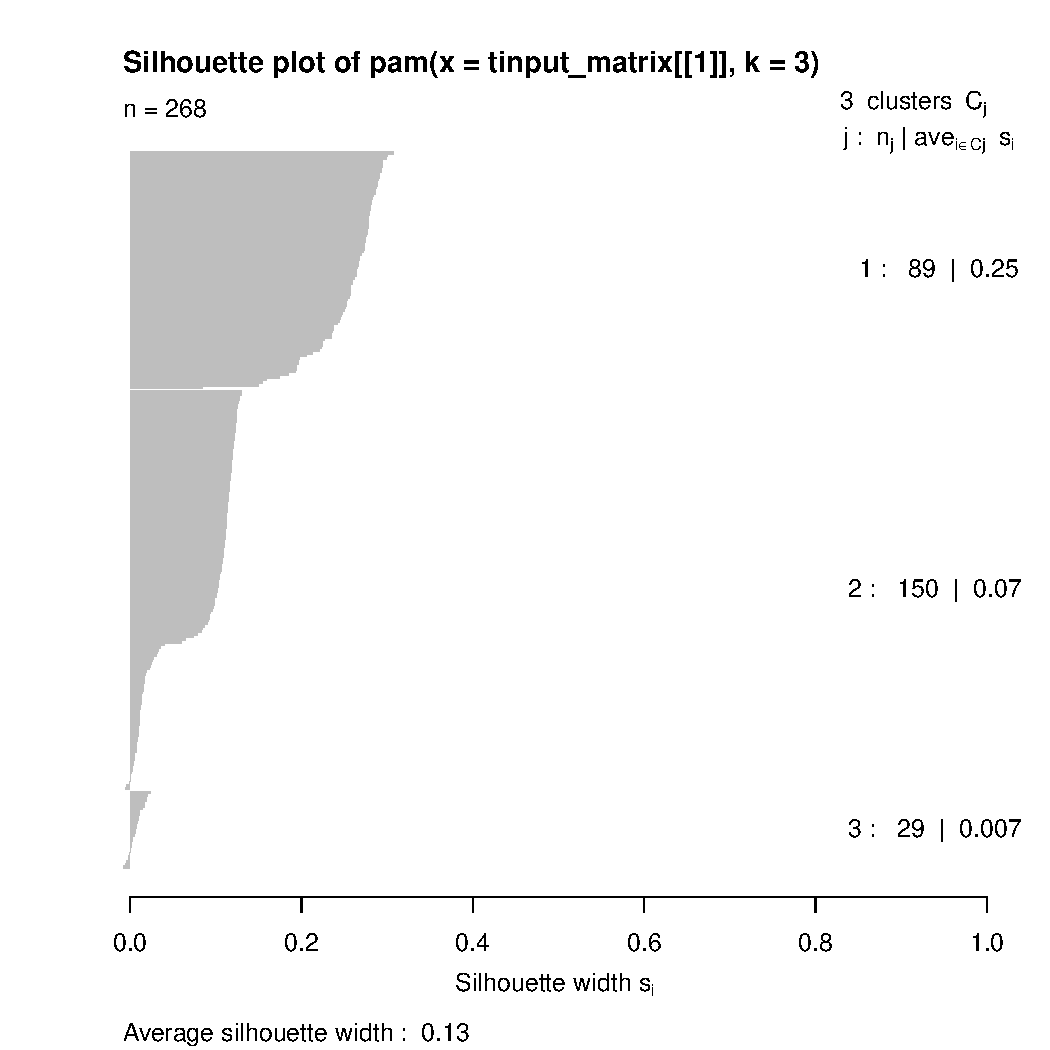
\includegraphics[width=5 in]{/Users/angeloduo/Desktop/masterarbeit/scRNAseq_clustering_comparison/results/plots/optimalk_wss.pdf}
\caption{Optimal number of clusters by within sum of squares based on the full dimensions }
\label{fig:wssorg}
\end{figure}



\begin{figure}[!h]
\includegraphics[width=5 in]{/Users/angeloduo/Desktop/masterarbeit/scRNAseq_clustering_comparison/results/QC_data/qc_summary_simDataKumar2.png}
\caption{QC summary of simDataKumar2. }
\label{fig:simDataKumar}
\end{figure}
\clearpage


\begin{figure}[!h]
\includegraphics[width=5 in]{/Users/angeloduo/Desktop/masterarbeit/scRNAseq_clustering_comparison/results/plots/plot_ari_smooth.pdf}
\caption{ARI scores with smoothed data sets.  }
\label{fig:arifilt}
\end{figure}




\begin{figure}[!h]
\includegraphics[width=5 in]{/Users/angeloduo/Desktop/masterarbeit/scRNAseq_clustering_comparison/results/plots/plot_ari_stars_all.pdf}
\caption{Starplot of ARI scores.  }
\label{fig:arirank}
\end{figure}







\begin{figure}[!h]
\includegraphics[width=5 in]{/Users/angeloduo/Desktop/masterarbeit/scRNAseq_clustering_comparison/results/plots/runtimes.pdf}
\caption{Runtime (s) for the methods on the datasets Kumar Trapnell, Zheng, Koh, simDataKumar and simDatakumar2. The datasets are filtered and the number of clusters based on the ground truth is used.}
\label{fig:runtime}
\end{figure}



\begin{figure}[!h]
\includegraphics[width=5 in]{/Users/angeloduo/Desktop/masterarbeit/scRNAseq_clustering_comparison/results/plots/stability_boot.pdf}
\caption{Stability analysis results with (20) bootstrap samples for the Kumar dataset.}
\label{fig:boot}
\end{figure}


\begin{figure}[!h]
\includegraphics[width=5 in]{/Users/angeloduo/Desktop/masterarbeit/scRNAseq_clustering_comparison/results/plots/plot_ari_unfiltered.pdf}
\caption{ARI scores with unfiltered data sets. The number of clusters is determined by the authors annotation. }
\label{fig:ariunfilt}
\end{figure}

\begin{figure}[!h]
\includegraphics[width=5 in]{/Users/angeloduo/Desktop/masterarbeit/scRNAseq_clustering_comparison/results/plots/plot_ari_default.pdf}
\caption{ARI scores with default setting. }
\label{fig:aridef}
\end{figure}

\begin{figure}[!h]
\includegraphics[width=5 in]{/Users/angeloduo/Desktop/masterarbeit/scRNAseq_clustering_comparison/results/plots/plot_ari_filtered.pdf}
\caption{ARI scores with filtered data sets.  The number of clusters is determined by the authors annotation. }
\label{fig:arifilt}
\end{figure}

\begin{figure}[!h]
\includegraphics[width=5 in]{/Users/angeloduo/Desktop/masterarbeit/scRNAseq_clustering_comparison/results/plots/plot_ari_optimalk.pdf}
\caption{ARI scores with filtered data sets. A optimal k is chosen such that the ARI score is maximized. }
\label{fig:ariopt}
\end{figure}






% Table generated by Excel2LaTeX from sheet 'Blatt2'
\begin{table}[htbp]
\centering
\caption{Add caption}
\begin{tabular}{llrr}
method & parameters & \multicolumn{1}{l}{default} & \multicolumn{1}{l}{annotated k} \\
cidr  & n     & \multicolumn{1}{l}{NULL} & \multicolumn{1}{l}{NULL} \\
cidr  & nCluster & \multicolumn{1}{l}{NULL} & \multicolumn{1}{l}{k} \\
cidr  & nPC   & 4     & 4 \\
cidr  & cMethod & \multicolumn{1}{l}{wardD2} & \multicolumn{1}{l}{wardD2} \\
dbscan & eps   & \multicolumn{1}{l}{user} & \multicolumn{1}{l}{user} \\
dbscan & minPts (kNN) & 5     & 0.1 \\
linnorm & minZeroPortion & 0.75  & \multicolumn{1}{l}{0.75 , (0.25 for Zheng)} \\
linnorm & num\_PC & 3     & 3 \\
linnorm & num\_Center & \multicolumn{1}{l}{1 to 20} & \multicolumn{1}{l}{k} \\
RaceID & min.total & \multicolumn{1}{l}{3000 ( 200 for Zheng)} & \multicolumn{1}{l}{3000 ( 200 for Zheng)} \\
RaceID & max.expr & \multicolumn{1}{l}{Inf} & \multicolumn{1}{l}{Inf} \\
RaceID & min.expr & 5     & 5 \\
RaceID & minnumber & 1     & 1 \\
RaceID & do.gap & \multicolumn{1}{l}{TRUE} & \multicolumn{1}{l}{FALSE} \\
RaceID & clustrnr & 20    & 0 \\
RaceID & cln   & 0     & \multicolumn{1}{l}{k} \\
Rtsnekmeans & k     & \multicolumn{1}{l}{k} & \multicolumn{1}{l}{k} \\
Rtsnekmeans & Perplexity & 30    & 30 \\
Rtsnekmeans & initial\_dims & 50    & 30 \\
SIMLRlargescale & c     & \multicolumn{1}{l}{k} & \multicolumn{1}{l}{k} \\
SIMLRlargescale & k     & 10    & 10 \\
SIMLRlargescale & kk    & 100   & 100 \\
SIMLRlargescale & normalize & \multicolumn{1}{l}{FALSE} & \multicolumn{1}{l}{FALSE} \\
SIMLR & c     & \multicolumn{1}{l}{k} & \multicolumn{1}{l}{k} \\
SIMLR & k     & 10    & 10 \\
SIMLR & kk    & 100   & 100 \\
SIMLR & normalize & \multicolumn{1}{l}{FALSE} & \multicolumn{1}{l}{TRUE} \\
SIMLR & no.dim & \multicolumn{1}{l}{NA} & \multicolumn{1}{l}{NA} \\
tscan & minexpr\_percent & \multicolumn{1}{p{7.25em}}{0.1 to 0.5} & \multicolumn{1}{p{10.835em}}{0.1 to 0.5} \\
tscan & clusternum & \multicolumn{1}{l}{2 to 20} & \multicolumn{1}{l}{k} \\
SC3   & ks    & \multicolumn{1}{l}{2 to 10} & \multicolumn{1}{l}{elbowplot} \\
SC3   & k\_estimator & \multicolumn{1}{l}{TRUE} & \multicolumn{1}{l}{FALSE} \\
SEURAT & k.param & 30    & \multicolumn{1}{l}{10 percent} \\
SEURAT & dims.use & \multicolumn{1}{l}{NULL} & \multicolumn{1}{p{10.835em}}{screeplot} \\
SEURAT & reduction.type & \multicolumn{1}{l}{pca} & \multicolumn{1}{l}{pca} \\
SEURAT & resolution  & 0.8   & 0.8 \\
pcaReduce & q     & 30    & 30 \\
pcaReduce & nbt   & 100   & 100 \\
\end{tabular}%
\label{tab:addlabel}%
\end{table}%

\clearpage
\begin{table}[ht]
\centering
\begin{tabular}{rllllll}
  \hline
 & method & parameters & default & annotated k & highest ARI (from k range) & X6 \\ 
  \hline
1 & cidr & n & NULL & NULL &  &  \\ 
  2 & cidr & nCluster & NULL & k &  &  \\ 
  3 & cidr & nPC & 4 & 4 &  &  \\ 
  4 & cidr & cMethod & wardD2 & wardD2 &  &  \\ 
  5 & dbscan & eps & user & user &  &  \\ 
  6 & dbscan & minPts (kNN) & 5 & 0.1 &  &  \\ 
  7 & linnorm & minZeroPortion & 0.75 & 0.75 , (0.25 for Zheng) &  &  \\ 
  8 & linnorm & num\_PC & 3 & 3 &  &  \\ 
  9 & linnorm & num\_Center & 1 to 20 & k &  &  \\ 
  10 & RaceID & min.total & 3000 ( 200 for Zheng) & 3000 ( 200 for Zheng) &  &  \\ 
  11 & RaceID & max.expr & Inf & Inf &  &  \\ 
  12 & RaceID & min.expr & 5 & 5 &  &  \\ 
  13 & RaceID & minnumber & 1 & 1 &  &  \\ 
  14 & RaceID & do.gap & TRUE & FALSE &  &  \\ 
  15 & RaceID & clustrnr & 20 & 0 &  &  \\ 
  16 & RaceID & cln & 0 & k &  &  \\ 
  17 & Rtsnekmeans & k & k & k &  &  \\ 
  18 & Rtsnekmeans & Perplexity & 30 & 30 &  &  \\ 
  19 & Rtsnekmeans & initial\_dims & 50 & 30 &  &  \\ 
  20 & SIMLRlargescale & c & k & k &  &  \\ 
  21 & SIMLRlargescale & k & 10 & 10 &  &  \\ 
  22 & SIMLRlargescale & kk & 100 & 100 &  &  \\ 
  23 & SIMLRlargescale & normalize & FALSE & FALSE &  &  \\ 
  24 & SIMLR & c & k & k &  &  \\ 
  25 & SIMLR & k & 10 & 10 &  &  \\ 
  26 & SIMLR & kk & 100 & 100 &  &  \\ 
  27 & SIMLR & normalize & FALSE & TRUE &  &  \\ 
  28 & SIMLR & no.dim &  &  &  &  \\ 
  29 & tscan & minexpr\_percent & 0.1 to 0.5 & 0.1 to 0.5 &  &  \\ 
  30 & tscan & clusternum & 2 to 20 & k &  &  \\ 
  31 & SC3 & ks & 2 to 10 & elbowplot &  &  \\ 
  32 & SC3 & k\_estimator & TRUE & FALSE &  &  \\ 
  33 & SEURAT & k.param & 30 & 10 percent &  &  \\ 
  34 & SEURAT & dims.use & NULL & screeplot &  &  \\ 
  35 & SEURAT & reduction.type & pca & pca &  &  \\ 
  36 & SEURAT & resolution & 0.8 & 0.8 &  &  \\ 
  37 & pcaReduce & q & 30 & 30 &  &  \\ 
  38 & pcaReduce & nbt & 100 & 100 &  &  \\ 
   \hline
\end{tabular}
\end{table}


\begin{kframe}


{\ttfamily\noindent\bfseries\color{errorcolor}{\#\# Error in `align<-.xtable`(`*tmp*`, value = switch(1 + is.null(align), : "{}align"{} must have length equal to 5 ( ncol(x) + 1 )}}\end{kframe}

\newpage

\begin{center}
\begin{table}[!h]
\footnotesize
\begin{tabular}{ | p{ 2 cm} |  p{ 5 cm}  | p{ 2 cm} | p{ 2 cm} | p{ 0.5 cm} | p{ 0.6 cm} | p{ 0.6 cm} |}
    \hline
    Method & Description & dimension reduction & clustering & zero inflation & normalization & unsupervised \\ \hline
    \hline
     tSNEkmeans & tSNE dimension reduction and kmeans clustering & tSNE & kmeans & no & no & no \\ \hline
    pcaReduce &PCA dimension reduction and kmeans clustering through an iterative process. Step wise merging of cluster by joint probabilities and reducing the number of dimension by PC with lowest variance & PCA & kmeans, hierarchical clustering & no & no &  \\ \hline
     SC3 & PCA  dimension reduction or Laplacian graph. Kmeans clustering on different dimensions. Hierarchical clustering on consensus matrix obtained by kmeans. & PCA & repeated kmeans, hierarchical clustering on similarity matrix of kmeans results & no & no & yes \\ \hline
    SNN-cliq & Shared nearest neighbor  graph based on similarities. Clustering through forming of cliques and subsequent merging. & graph based & merging of cliques & no & no &  \\ \hline
        dbscan & Density based clustering & none &density based clustering & no & no & yes \\ \hline
     SIMLR &  & tSNE & kmeans & yes & no & yes \\ \hline
    CIDR & PCA dimension reduction based on zero imputed similarities. Hierarchical clustering on a number of PC determined by variation of scree method. & PCA on imputed distances & hierarchical clustering& yes & no & yes \\ \hline
   Seurat v1.4 & Nearest neighbor graph based on PCA latent space & HVG and PCA & & no & yes & yes \\ \hline


    \end{tabular}
    \end{table}
\end{center}

Only the methods SC3, and SIMLR (for large-scale data) were able to identify cell population 1. 
The proportions of differentially expressed genes are relatively low for three out of the four subgroups, and these populations are relatively distinct. 
However, RaceID and pcaReduce had substantially lower ARI scores in the default setting.  It is unclear why pcaReduce and RaceID performed badly under the default setting.and most methods were able to identify these three clusters correctly
 Most methods achieved high F1 scores for subpopulation 1. The scores were substantially lower for the subpopulations 2 and 3an  TSCAN failed to identify the subpopulation 3.
The Koh dataset had the highest number of clusters of the studied datasets.  Here, only the methods SC3 and Seurat achieved an almost perfect partition of the cells.  



% =======================================
% \section{References} \label{sec:ref}
% =======================================
\clearpage

\bibliography{/Users/angeloduo/Desktop/masterarbeit/scRNAseq_clustering_comparison/report/scRNAseq_clustering.bib}


\end{document}
